% !TEX TS-program = lualatex
\documentclass[12pt,a4paper]{article}

\setlength{\parskip}{\medskipamount}
\setlength{\parindent}{0pt}
\usepackage{array}
\usepackage{graphicx}
\usepackage{multicol}
\usepackage[dvipsnames]{xcolor}
\usepackage{colortbl}
\usepackage[yyyymmdd,hhmmss]{datetime}
\usepackage{lastpage}
\providecommand{\tabularnewline}{\\}
\newcommand{\PreserveBackslash}[1]{\let\temp=\\#1\let\\=\temp}
\let\PBS=\PreserveBackslash
\usepackage{setspace}
\usepackage{multirow}
%% end paste
\usepackage{amssymb,amsmath}
%\usepackage{ifluatex}

% use upquote if available, for straight quotes in verbatim environments
\IfFileExists{upquote.sty}{\usepackage{upquote}}{}
% use microtype if available
\IfFileExists{microtype.sty}{%
\usepackage{microtype}
\UseMicrotypeSet[protrusion]{basicmath} % disable protrusion for tt fonts
}{}
\usepackage[includehead,includefoot]{geometry}
\geometry{lmargin=1in,rmargin=1in,tmargin=0.75in,
bmargin=1.0in,headheight=0pt,headsep=0pt,marginparwidth=0pt,
footskip=2.5\baselineskip,
}
\usepackage{hyperref}
\PassOptionsToPackage{usenames,dvipsnames}{color} % color is loaded by hyperref
%% Control hyperlink colours

\usepackage{hyperref}

\hypersetup{
    colorlinks=true,    % Enable colored links
    linkcolor=oupred,
    citecolor=black,
    urlcolor=oupred,
    pdfborder={0 0 0}   % Remove borders around links
}

\urlstyle{same}  % don't use monospace font for urls


\usepackage[style=apa, natbib=true]{biblatex}

\addbibresource{~/Library/CloudStorage/OneDrive-UniversityofWarwick/Warwick/Modules/PO91Q/referencesPO91Q.bib}
\usepackage{listings}
\newcommand{\passthrough}[1]{#1}
\usepackage{longtable,booktabs, dcolumn}
\usepackage{graphicx,grffile}
\usepackage{fancyhdr}
\lhead{}
\chead{}
\rhead{}
\renewcommand{\headrulewidth}{0pt}
\lfoot{}
\cfoot{{Page} \thepage { of} \pageref{LastPage}}
\rfoot{}

\fancypagestyle{firststyle}
{
\lfoot{}
% \cfoot{{Page} \thepage { of} \pageref{LastPage}}
\cfoot{}
\rfoot{}
\renewcommand{\headrulewidth}{0pt}
\fancyfoot[L]{}
\fancyfoot[R]{}
}

\pagestyle{fancy}
\thispagestyle{firststyle}

\makeatletter
%graphics and such inside floats are centered by default
\renewenvironment{figure}[1][]{%
 \ifthenelse{\equal{#1}{}}{%
   \@float{figure}
 }{%
   \@float{figure}[#1]%
 }%
 \centering
}{%
 \end@float
}
\renewenvironment{table}[1][]{%
 \ifthenelse{\equal{#1}{}}{%
   \@float{table}
 }{%
   \@float{table}[#1]%
 }%
 \centering
}{%
 \end@float
}
\makeatother

\usepackage{titlesec}
\newcommand{\hsp}{\hspace{20pt}}

% ===== Headings (unchanged) =====
\titleformat{\section}[hang]
  {\fontsize{15pt}{16pt}\selectfont}
  {\thesection\hsp\textcolor{gray!75}{|}\hsp}{0pt}{}

\titleformat{\subsection}[hang]
  {\fontsize{12pt}{12pt}\selectfont}
  {\thesubsection\hsp}{0pt}{}

\titleformat{\subsubsection}[hang]
  {\fontsize{11pt}{11pt}\selectfont}
  {\thesubsubsection\hsp}{0pt}{}
  [{\vspace{-1.0ex}}]  % reduces vertical space after subsection heading

% ===== Parts (unchanged) =====
\titleformat{\part}[block]
  {\normalfont\large\bfseries}
  {Part \thepart:}{1em}{}
\titlespacing*{\part}{0pt}{2ex}{3ex}

% ===== TOC: consistent indentation (deeper levels = further in) =====
% \@dottedtocline{level}{indent}{numwidth}
% Keep your overall look but make L2/L3 indented relative to L1.
\makeatletter
% \@dottedtocline{level}{indent}{numwidth}
% Slightly smaller indents and numwidths for a tighter look
\renewcommand{\l@section}      {\@dottedtocline{1}{1.2em}{1.5em}}  % level-1
\renewcommand{\l@subsection}   {\@dottedtocline{2}{2.7em}{2.5em}}  % level-2
\renewcommand{\l@subsubsection}{\@dottedtocline{3}{5.2em}{2.5em}}  % level-3
\makeatother


% ===== TOC: part entry styling (unchanged) =====
\makeatletter
\renewcommand{\l@part}[2]{%
  \vskip 10pt
  \begingroup
    \small\bfseries
    \@tempdima 3em
    \parindent \z@ \rightskip \@pnumwidth
    \parfillskip -\@pnumwidth
    \leavevmode
    \advance\leftskip\@tempdima
    \hskip -\leftskip
    #1\nobreak\hfil \nobreak\hb@xt@\@pnumwidth{\hss #2}\par
  \endgroup
}
\makeatother


%[{\vspace{1.0ex}\titlerule[1.5pt]}] %includes a rule under the heading

%% Eliminate reliance on Sweavel or Sweave
%% \usepackage{Sweavel}
%% \usepackage[noae]{Sweave}
\usepackage{listings}
\usepackage{upquote, fancyvrb, relsize, ae}

%%\lstset{tabsize=2, breaklines=true,style=Rstyle}
\definecolor{darkgreen}{RGB}{0,100,0}
\definecolor{indianred}{RGB}{205,92,92}
\definecolor{darkmagenta}{RGB}{104,34,139}
\definecolor{steelblue}{RGB}{70,130,180}
\definecolor{steelblue1}{RGB}{130,150,190}
\definecolor{frameblue}{RGB}{20,40,80}
\definecolor{antwhite}{RGB}{139,119,101}
\definecolor{lightgray}{RGB}{240,240,240}
\definecolor{darkblue}{HTML}{1e2277}
\definecolor{kublue81186}{RGB}{0,81,186}


% Format Dates
\newdateformat{monddyyy}{\shortmonthname[\THEMONTH].~\THEDAY,~\THEYEAR}



%%%%%%%%%%%%%%%%%%%%%%%%%%%%%%%%%%%%%%%%%%%%%%%%%%%%%%%%%%%%%%%%%%%%%%%%%%%%%%%%%%%%%%%%%%%%%%%%%%%%%%%%%%%%%%%%%%%%%%%%%%%%%%%%%%%%%%%%%%%%%%%%%%%%%%%%%%%%%%%%%%%%%%%%%%%%%%%%%%%%%%%%%%%%%%
% F O R M A T T I N G   F O R   C O D E   C H U N K S %
%%%%%%%%%%%%%%%%%%%%%%%%%%%%%%%%%%%%%%%%%%%%%%%%%%%%%%%%%%%%%%%%%%%%%%%%%%%%%%%%%%%%%%%%%%%%%%%%%%%%%%%%%%%%%%%%%%%%%%%%%%%%%%%%%%%%%%%%%%%%%%%%%%%%%%%%%%%%%%%%%%%%%%%%%%%%%%%%%%%%%%%%%%%%%%%
\def\Sweavesize{\scriptsize} 
\def\Rcolor{\color{black}} 
\def\Rbackground{\color{oupgrey45}}


\lstdefinestyle{Rstylecrmda}{
  language=R,
  escapechar=`,
  fancyvrb=false,
  tabsize=2,
  breaklines=true,
  linewidth=\linewidth,
  breakatwhitespace=false,
  captionpos=b,
  frame=leftline,
  rulecolor=\color{oupred},
  showstringspaces=false,
  backgroundcolor=\Rbackground,
  columns=fixed,
  basicstyle=\linespread{1.5}\ttfamily\upshape,
  identifierstyle=\linespread{1.5}\ttfamily\upshape,
  keywordstyle=\linespread{1.5}\ttfamily\upshape,
  stringstyle=\linespread{1.5}\ttfamily\upshape,
  commentstyle=\linespread{1.5}\ttfamily\upshape,
  escapeinside={(*}{*)},
  literate={~}{{$\sim$}}1 {==}{{=\,=}}2,
  alsoother={$},
  alsoletter={.<-},
  otherkeywords={!,!=,~,$,*,\&,\%/\%,\%*\%,\%\%,<-,<<-,/},
}

\makeatletter
\renewcommand*\verbatim@nolig@list{}
\makeatother

\lstset{style=Rstylecrmda}



% exact size for inline code via listings
\lstdefinestyle{InlineCode}{
  basicstyle={\ttfamily\fontsize{9pt}{10.8pt}\selectfont}
}
\let\Oldlstinline\lstinline
\DeclareRobustCommand{\lstinline}[1][]{\Oldlstinline[style=InlineCode,#1]}


\makeatletter
\def\maxwidth{\ifdim\Gin@nat@width>\linewidth\linewidth\else\Gin@nat@width\fi}
\def\maxheight{\ifdim\Gin@nat@height>\textheight\textheight\else\Gin@nat@height\fi}
\makeatother
% Scale images if necessary, so that they will not overflow the page
% margins by default, and it is still possible to overwrite the defaults
% using explicit options in \includegraphics[width, height, ...]{}
\setkeys{Gin}{width=\maxwidth,height=\maxheight,keepaspectratio}
\IfFileExists{parskip.sty}{%
\usepackage{parskip}
}{% else
\setlength{\parindent}{0pt}
\setlength{\parskip}{6pt plus 2pt minus 1pt}
}
\setlength{\emergencystretch}{3em}  % prevent overfull lines
\providecommand{\tightlist}{%
  \setlength{\itemsep}{0pt}\setlength{\parskip}{0pt}}
\setcounter{secnumdepth}{0}
% Redefines (sub)paragraphs to behave more like sections
\ifx\paragraph\undefined\else
\let\oldparagraph\paragraph
\renewcommand{\paragraph}[1]{\oldparagraph{#1}\mbox{}}
\fi
\ifx\subparagraph\undefined\else
\let\oldsubparagraph\subparagraph
\renewcommand{\subparagraph}[1]{\oldsubparagraph{#1}\mbox{}}
\fi

%%% Use protect on footnotes to avoid problems with footnotes in titles
\let\rmarkdownfootnote\footnote%
\def\footnote{\protect\rmarkdownfootnote}


% %   \title{PO91Q: Fundamentals in Quantitative Research Methods}
%   % % % \subtitle{Week 5 - Solutions}
% % %   \author{true \\ true}
%   % % %   \date{}
%   % 
%\usepackage[T1]{fontenc} \usepackage{lmodern}
\providecommand{\passthrough}[1]{#1}
\usepackage{calc,array}
\usepackage{booktabs}
\usepackage{ragged2e}
\usepackage{tabularx,calc}
\usepackage{longtable}
\usepackage{dcolumn}
\usepackage{graphicx}
\usepackage{amsmath, amsthm, amssymb}
\usepackage{mathtools}
\usepackage{dsfont}
\usepackage{listings}
\usepackage{multirow}
\usepackage{multicol}
\usepackage{url}
\usepackage{rotating}
\usepackage{tabularx}
%\usepackage[dvipsnames]{xcolor}
\usepackage{subfig}
\usepackage{placeins}
%\usepackage{subfigure}
%\definecolor{heading}{RGB}{235, 125, 52}
%\renewcommand{\familydefault}{\sfdefault}
\usepackage[most]{tcolorbox}
%\tcbset{colback={rgb,255:red,251;green,236;blue,200}, colframe={rgb,255:red,157;green,34;blue,53}}
%\tcbset{colback={rgb,255:red,235;green,205;blue,150}, colframe={rgb,255:red,214;green,154;blue,45}}
%\tcbset{colback={rgb,255:red,235;green,205;blue,150}, colframe={rgb,255:red,214;green,154;blue,45}}
\usepackage{bm}
\usepackage{placeins}
\usepackage{float}
\usepackage{etoolbox}
\tcbuselibrary{theorems}
\usepackage{pdflscape}
\newcolumntype{L}{>{\raggedright\arraybackslash}X}
\newcolumntype{R}{>{\raggedleft\arraybackslash}X}
\newcolumntype{Y}{>{\raggedleft\arraybackslash}X}
\newcolumntype{C}{>{\centering\arraybackslash}X}
\newcolumntype{b}{C}
\newcolumntype{s}{>{\hsize=.333\hsize}b}
\floatplacement{figure}{H}
\usepackage{makecell}
\usepackage{caption}
\captionsetup[longtable]{position=bottom}

%\usepackage{scrextend}
%\addtokomafont{labelinglabel}{\sffamily\bfseries}



% Allow line breaks in verbatim
\usepackage{fancyvrb}
\usepackage{fvextra}
\fvset{breaklines=true}

\usepackage{csquotes}

\usepackage{tasks}
\usepackage{mdframed}
%\definecolor{waraubergine}{RGB}{85, 45, 98} %this IS right
\definecolor{waraubergine}{RGB}{60, 15, 83} %this looks right
\colorlet{shadecolor}{waraubergine!10}

% Strike through text
\usepackage{soul} %st{}


%LITTLE FILE CARDS
\usepackage{varwidth}
\newtcolorbox{mybox}[2][]{enhanced, interior hidden,
before=\par\smallskip\centering,
colframe=wargolddark!50, colback=wargolddark!50, coltitle=black,
fonttitle=\bfseries\sffamily,
attach boxed title to top left,
boxed title style={empty, boxrule=0.5mm},
varwidth boxed title=0.5\linewidth,
underlay boxed title={
\path[draw=wargolddark!50, line width=0.5mm, rounded corners, fill=wargolddark!50]
([xshift=.25mm]frame.west) |- ([xshift=-2.5mm]title.north east) to[out=0, in=180] ([xshift=7.5mm, yshift=-.25mm]title.south east);  
},
title={#2},#1}

% format coloured lines in tables
\usepackage{arydshln}
\newcommand\VRule[1][\arrayrulewidth]{\vrule width #1}






% Some optional colors.
%---------------------------------------------------
%include other Warwick Colours
\definecolor{warruby}{RGB}{157,34,53}
\definecolor{warruby25}{RGB}{231,200,205}
\definecolor{warorange}{RGB}{190,83,28}
\definecolor{wargold}{RGB}{241,190,72}
\definecolor{wargolddark}{RGB}{214,154,45}
\definecolor{warblue}{RGB}{0,169,206}
\definecolor{warbluedark}{RGB}{65,116,141}
\definecolor{quotegrey}{RGB}{153,153,153} 

%include OUP Colours
\definecolor{oupred}{RGB}{138,30,0} 
\definecolor{oupred75}{RGB}{167,86,64} 
\definecolor{oupred50}{RGB}{197,143,128} 
\definecolor{oupred25}{RGB}{226,199,191} 
\definecolor{oupred20}{RGB}{232,210,204} 
\definecolor{oupred15}{RGB}{237,221,217}

\definecolor{ouporange}{RGB}{229,119,38} 
\definecolor{ouporange75}{RGB}{236,153,92} 
\definecolor{ouporange50}{RGB}{242,187,147} 
\definecolor{ouporange25}{RGB}{249,221,201} 
\definecolor{ouporange15}{RGB}{251,235,222} 

\definecolor{oupbrown}{RGB}{190,90,22} 
\definecolor{oupbrown25}{RGB}{239,214,197}

\definecolor{oupgrey}{RGB}{145,146,148} 
\definecolor{oupgrey75}{RGB}{173,173,175} 
\definecolor{oupgrey50}{RGB}{200,201,202}
\definecolor{oupgrey45}{RGB}{206,206,207}

%maths box colour
\tcbset{
  mymathstyle/.style={
    colback={rgb,255:red,236;green,203;blue,187}, % Background color
    boxrule=0mm,                                  % No border around the box
    enhanced,                                     % Enable advanced settings like borderline
    borderline west={0.8mm}{0pt}{warorange},      % Add a vertical line on the left (west)
    sharp corners                                 % Ensure sharp rectangular corners
  }
}

% Apply the style only to \tcboxmath
\renewcommand{\tcboxmath}[1]{\tcbhighmath[mymathstyle]{#1}}


%%%%%%%%%%%%%%%%%%%%%%%%%%%%%%%%%%%%%%%%%%%%%%%%%%%%%%%%%%%%%%%%%%%%%%%%%%%
% F O R M A T T I N G   F O R   C O D E   C H U N K S %
%%%%%%%%%%%%%%%%%%%%%%%%%%%%%%%%%%%%%%%%%%%%%%%%%%%%%%%%%%%%%%%%%%%%%%%%%%%

%\usepackage[dvipsnames]{xcolor}
%\usepackage[rgb]{xcolor}
\usepackage{tikz}
\usepackage{pgfplots}
\pgfplotsset{compat=1.18}
\usetikzlibrary{arrows.meta, matrix, calc}
\usetikzlibrary{positioning}
\usetikzlibrary{decorations.pathreplacing}
%
%\colorlet{shadecolor}{oupred20}



\usepackage{siunitx}


% Personalised Toprule and Bottomrule
\usepackage{ctable} % for \specialrule command
\newcommand\T{\specialrule{.08em}{.05em}{.17em}\hline} % Top Rule
\newcommand\B{\hline\specialrule{.08em}{.17em}{.05em}} % Bottom Rule


% Place captions underneath modelsummary tables
\usepackage{tabularray}
\DefTblrTemplate{firsthead,middlehead,lasthead}{default}{}
\DefTblrTemplate{firstfoot,middlefoot}{default}{}
\DefTblrTemplate{lastfoot}{default}% 
{
  \UseTblrTemplate{note}{default}
  \UseTblrTemplate{caption}{default}
}



%\usepackage{emoji}

% allow floats to be moved around
\usepackage{changepage}

% define my own checkmark
\usepackage{bbding}


% create a toolbox
\newtcbtheorem{toolbox}{Toolbox}{
colback=oupbrown25,              % Background color of the box
  colframe=white,               % No visible frame
  coltitle=white,               % Color of the title text
  colbacktitle=oupbrown, 		% Background color of the title area
  fonttitle=\bfseries,          % Bold title text
  left=4mm,                     % Space on the left-hand side for the line
  sharp corners,                % Remove rounded corners
  borderline west={5pt}{0pt}{oupbrown}, % Solid line on the left-hand side
  enhanced,                     % Enable extra tcolorbox features
  frame hidden,                 % Hide the main frame
  boxrule=0pt,                  % No box borders
  title after break={},         % To ensure title appears correctly
  before skip=10pt,             % Space before the box
  after skip=10pt,}{tb}
  
  
% make pandocbounded work

\usepackage{graphicx}
\usepackage{adjustbox}
\providecommand{\pandocbounded}[1]{%
  \begin{adjustbox}{max size={.95\linewidth}{.95\textheight}}#1\end{adjustbox}%
}

\pagecolor{lightgray}
\renewcommand{\toprule}{\specialrule{.08em}{.05em}{.17em}\hline}
\renewcommand{\bottomrule}{\hline\specialrule{.08em}{.17em}{.05em}}
\makeatletter
\@ifpackageloaded{caption}{}{\usepackage{caption}}
\AtBeginDocument{%
\ifdefined\contentsname
  \renewcommand*\contentsname{Table of contents}
\else
  \newcommand\contentsname{Table of contents}
\fi
\ifdefined\listfigurename
  \renewcommand*\listfigurename{List of Figures}
\else
  \newcommand\listfigurename{List of Figures}
\fi
\ifdefined\listtablename
  \renewcommand*\listtablename{List of Tables}
\else
  \newcommand\listtablename{List of Tables}
\fi
\ifdefined\figurename
  \renewcommand*\figurename{Figure}
\else
  \newcommand\figurename{Figure}
\fi
\ifdefined\tablename
  \renewcommand*\tablename{Table}
\else
  \newcommand\tablename{Table}
\fi
}
\newcommand*\listoflistings\lstlistoflistings
\AtBeginDocument{%
\renewcommand*\lstlistlistingname{List of Listings}
}
\makeatother
\makeatletter
\makeatother
\makeatletter
\@ifpackageloaded{caption}{}{\usepackage{caption}}
\@ifpackageloaded{subcaption}{}{\usepackage{subcaption}}
\makeatother



\usepackage{fontspec}

\setmainfont[Ligatures=TeX,
			 ItalicFont=*,ItalicFeatures=FakeSlant,
			 ]{FS Me}


\usepackage{isomath}

%allow changes in fornt size from YAML
\makeatletter
\renewcommand\normalsize{%
\@setfontsize\normalsize{10pt}{12pt}% Will look incredibly crabbed if line height is too small
\abovedisplayskip 10\p@ \@plus2\p@ \@minus5\p@%
\abovedisplayshortskip \z@ \@plus2\p@%
\belowdisplayshortskip 5\p@ \@plus2\p@ \@minus3\p@%
\belowdisplayskip \abovedisplayskip%
\let\@listi\@listI%
}
\normalsize  
\makeatother

%% SET FONT FOR CODE CHUNKS

\setmonofont{Gintronic}[Contextuals = Alternate,
    Ligatures = TeX,]


%% SET MATHS FONT


\usepackage{unicode-math}	

\setmathfont[Ligatures=TeX ,
			 ]{FiraMath-Regular} 
			 
\setmathfont{TeX Gyre DejaVu Math}[range={\vdots,\ddots}] 
			 

\usepackage{adjustbox}

\usepackage{eso-pic}

\AddToShipoutPictureBG*{%
  \AtPageLowerLeft{%
    \raisebox{1cm}{% Raise above bottom of page by 1cm
      \hspace*{\dimexpr\paperwidth - 0.375\textwidth}%
      \includegraphics[width=0.22\textwidth]{~/Dropbox/Markdown/Text.png}%
    }%
  }%
}

% vertical space between bibliography entries

\usepackage{etoolbox}

\AtBeginBibliography{%
  \setlength{\itemsep}{0.5em}  % space between entries
  \setlength{\parskip}{0pt}               % prevent extra spacing between lines
  \setlength{\parsep}{0pt}
}

% Patch the biblatex macro to wrap each entry in a samepage environment
\apptocmd{\bibitem}{\begin{samepage}}{}{}
\apptocmd{\endbibitem}{\end{samepage}}{}{}


\usepackage{xcolor}
\definecolor{waraubergine}{RGB}{60, 15, 83} %this looks right

\newtcolorbox{Rbox}[1][]{
  enhanced,
  breakable,
  width=\linewidth,
  frame hidden,
  borderline west={1.2pt}{0pt}{oupred}, % like frame=leftline + rulecolor
  colback=oupgrey45,                     % matches your \Rbackground look
  sharp corners,
  boxsep=1mm,
  left=3mm, right=2mm, top=1mm, bottom=1mm,
  fontupper=\linespread{1.5}\ttfamily\upshape,
  #1
}


% ================================
% BEGIN DOCUMENT
% ================================
% --------------------------------

\begin{document}

\begin{minipage}[t]{\textwidth}%
  \begin{center}
    \setlength{\arrayrulewidth}{1.5pt}

    % top colored rule
    {\color{waraubergine}\rule{\textwidth}{\arrayrulewidth}}

    \vspace{2pt}

    % --- two-column header row (75% / 24%) ---
    \begin{minipage}[t]{0.75\linewidth}
      \parbox[t]{\linewidth}{
                  \vspace{0.5ex}%
          {\textsc{\fontsize{13}{14}\selectfont PO91Q: Fundamentals in
Quantitative Research Methods}}
        
                  \par\vspace{1ex}%
          {\textsc{\fontsize{11}{12}\selectfont Week 5 - Solutions}}
        
        \vspace{1.5ex}

        \textcolor{waraubergine}{\rule[0.75ex]{0.75\textwidth}{1.0pt}}

        \vspace{1ex}

  \noindent Dr Florian Linke
  
  \noindent 
  \par\vspace{0.4ex}
    {\fontsize{10}{12}\selectfont
      \href{mailto:Florian.Linke@warwick.ac.uk}{\nolinkurl{Florian.Linke@warwick.ac.uk}}%
    }
  \par\vspace{1ex}


      }
    \end{minipage}\hfill
    \begin{minipage}[t]{0.24\linewidth}
      \centering
      \vspace{2ex}
      
\includegraphics[width=0.4\textwidth]{/Users/u1373867/Dropbox/Markdown/Crest.png}
      \vspace{4ex}
    \end{minipage}

    \vspace{2pt}

    % bottom colored rule
    {\color{waraubergine}\rule{\textwidth}{\arrayrulewidth}}
  \end{center}
  \medskip{}
\end{minipage}






\onehalfspacing

\section*{Effect size, sample size, and
power}\label{effect-size-sample-size-and-power}
\addcontentsline{toc}{section}{Effect size, sample size, and power}

\begin{enumerate}
\def\labelenumi{\arabic{enumi}.}
\tightlist
\item
  Same effect size, different n (mapping \(t\), \(n\), and \(\hat d\))

  \begin{enumerate}
  \def\labelenumii{\alph{enumii}.}
  \tightlist
  \item
    With \(t=1.6\) and \(n=16\), \(\hat d = t/\sqrt{n} = 1.6/4 = 0.40\).
    The power at \(n=16\) for \(\hat d \approx 0.40\) and
    \(\alpha=0.05\) will be modest (typically well below \(0.80\)).
  \item
    Keeping \(\hat d\) fixed at \(0.40\) and raising \(n\) to \(64\)
    requires \(t = \hat d \sqrt{n} = 0.40 \times 8 = 3.2\). The app will
    show the same \(\hat d\) but a higher power at \(n=64\).
  \item
    As \(n\) increases while the underlying effect stays fixed, the
    standard error shrinks: \(\mathrm{SE} = s/\sqrt{n}\). The test
    statistic is \(t = \dfrac{\bar{x}-\mu_0}{\mathrm{SE}}\), so a
    smaller \(\mathrm{SE}\) makes \(|t|\) larger on average. For a fixed
    \(\alpha\), the critical cutoff (e.g., \(t_{\alpha/2,\,df}\) for a
    two-sided test) is essentially fixed, so larger typical \(|t|\)
    increases the chance that \(|t| > t_{\alpha/2,\,df}\). Therefore,
    bigger \(n \Rightarrow\) less sampling noise \(\Rightarrow\) tighter
    estimates \(\Rightarrow\) higher power.
  \end{enumerate}
\end{enumerate}

\bigskip

\begin{enumerate}
\def\labelenumi{\arabic{enumi}.}
\setcounter{enumi}{1}
\tightlist
\item
  Planning with a SESOI and \(\alpha\) sensitivity

  \begin{enumerate}
  \def\labelenumii{\alph{enumii}.}
  \tightlist
  \item
    For \(t=2.0\) and \(n=30\),
    \(\hat d = t/\sqrt{n} \approx 2.0/\sqrt{30} \approx 0.37\). The app
    will report the power at \(n=30\) using this \(\hat d\) (typically
    moderate at \(\alpha=0.05\)).
  \item
    Turning on the SESOI with \(d=0.5\) switches the curve to a fixed
    target effect. The orange marker shows the \(n\) giving \(80\%\)
    power at \(\alpha=0.05\); for \(d=0.5\) this is typically in the
    few--dozen range for a one-sample \(t\)-test (on the order of the
    30s).
  \item
    Increasing \(\alpha\) to \(0.10\) lowers the critical threshold and
    reduces the required \(n\) for a given power; decreasing \(\alpha\)
    to \(0.01\) raises the threshold and increases the required \(n\).
    Formally, stricter \(\alpha\) increases the critical \(t\) value, so
    a larger \(n\) is needed for the same probability of exceeding it
    under the alternative.
  \end{enumerate}
\end{enumerate}

\bigskip

\begin{enumerate}
\def\labelenumi{\arabic{enumi}.}
\setcounter{enumi}{2}
\tightlist
\item
  Was the study well powered? Post-hoc check and replication planning

  \begin{enumerate}
  \def\labelenumii{\alph{enumii}.}
  \tightlist
  \item
    With \(t=2.1\) and \(n=25\),
    \(\hat d = 2.1/\sqrt{25} = 2.1/5 = 0.42\). The app will show the
    power at \(n=25\) for \(\hat d \approx 0.42\) and \(\alpha=0.05\);
    this is typically only moderate, not comfortably high.
  \item
    For replication planning, turn on SESOI and choose the closest
    option to \(\hat d\) (e.g., \(d=0.5\)). The orange marker will give
    the \(n\) needed for \(80\%\) power at the chosen \(\alpha\); expect
    a sample size in the few--dozen range for \(d=0.5\) at
    \(\alpha=0.05\).
  \item
    A significant result with low power can be fragile because small
    shifts in sampling may miss the effect and estimates are noisier.
    Picking a SESOI (a target \(d\) tied to practical importance) and
    planning for \(80\%\) power helps ensure a replication has adequate
    sensitivity to detect a meaningfully sized effect.
  \end{enumerate}
\end{enumerate}

\begin{tcolorbox}[
  enhanced,
  colback=oupred!30,          % 30% oupred background
  frame hidden,               % hide all borders
  borderline west={4pt}{0pt}{oupred} % thick right border only
]
Summarising Conclusions
\begin{itemize}
\item Power is the probability your test will detect a real effect (reject $H_0$ when the effect truly exists).
\item The curve fixes an effect size $d$ and shows how power increases with $n$.
\item If you base $d$ on your observed test ($\hat d = t/\sqrt{n}$), the curve answers: "If the effect really was the size we observed, how likely would the test be to detect that effect at other sample sizes $n$?"
\item If you base $d$ on a meaningful minimum (SESOI), the curve answers: "How large should $n$ be to reliably detect an effect that actually matters?"
\item The 0.80 (80\%) line is a convention (not a law). Many fields use it as a planning minimum; higher power (e.g., 90\%) is desirable when stakes are high.
\item Rule of thumb: because $t = d\sqrt{n}$, halving $d$ requires about 4× the sample size to keep power roughly the same.
\end{itemize}

\bigskip
Why do many plots show an 80\% power line?
\begin{itemize}
\item 80\% power means choosing $\beta = 0.20$ (so $\text{power} = 1 - \beta = 0.80$). This is a planning convention, not a mathematical law.
\item The convention became common through methodological guidance (e.g., Cohen’s power analysis texts) and is echoed in many applied fields.
\item In higher-stakes settings (e.g., confirmatory clinical trials), targets of 80–90\% power are typical; 90% is often preferred when feasible.
\end{itemize}
\end{tcolorbox}

\newpage

\section*{Case Study: Alcohol-Related Hospital Admissions and Mortality
in
Scotland}\label{case-study-alcohol-related-hospital-admissions-and-mortality-in-scotland}
\addcontentsline{toc}{section}{Case Study: Alcohol-Related Hospital
Admissions and Mortality in Scotland}

\subsection{Data Exploration}\label{data-exploration}

Before starting, we need to load libraries and install packages if not
already installed. In these exercises we will be using the
\texttt{tidyverse} package.

\begin{enumerate}
\def\labelenumi{\arabic{enumi}.}
\tightlist
\item
  Set your working directory, place the data set in it, and load it into
  R.
\item
  Create a new RScript for this case study and annotate it as you go
  through the exercises presented here.
\item
  Load the \texttt{tidyverse} package.
\end{enumerate}

\fontsize{7}{7}\selectfont
\normalsize

\subsection{\texorpdfstring{Descriptive
Statistics\label{sec:descr}}{Descriptive Statistics}}\label{descriptive-statistics}

\begin{enumerate}
\def\labelenumi{\arabic{enumi}.}
\tightlist
\item
  Produce descriptive statistics for all three numerical variables.
\end{enumerate}

\fontsize{7}{7}\selectfont

\begin{lstlisting}[language=R]
summary(simd$alc16)
##    Min. 1st Qu.  Median    Mean 3rd Qu.    Max. 
##   48.15   66.83   99.03   98.71  116.07  205.29
\end{lstlisting}

\normalsize

\fontsize{7}{7}\selectfont

\begin{lstlisting}[language=R]
summary(simd$mortality16)
##    Min. 1st Qu.  Median    Mean 3rd Qu.    Max. 
##   79.04   89.49   94.86   96.72  103.17  126.68
\end{lstlisting}

\normalsize

\fontsize{7}{7}\selectfont

\begin{lstlisting}[language=R]
summary(simd$mortality20)
##    Min. 1st Qu.  Median    Mean 3rd Qu.    Max.    NA's 
##   79.09   89.82   94.26   95.58  100.79  113.59       1
\end{lstlisting}

\normalsize

\subsection{Visualisation}\label{visualisation}

Let's visualise the distribution of the variable \texttt{alc16}.

\fontsize{7}{7}\selectfont

\begin{lstlisting}[language=R]
ggplot(simd, aes(x=alc16)) +
  geom_density(aes(y=..density..)) +
  theme_classic() +
  scale_x_continuous(name="Alcohol-Related Hospital Admissions (2011-2014)")+
  ylab('Density') +
  theme(axis.text=element_text(size=12),
        axis.title=element_text(size=13))
\end{lstlisting}

\normalsize

\fontsize{7}{7}\selectfont
\normalsize

\fontsize{7}{7}\selectfont

\begin{figure}[H]

{\centering 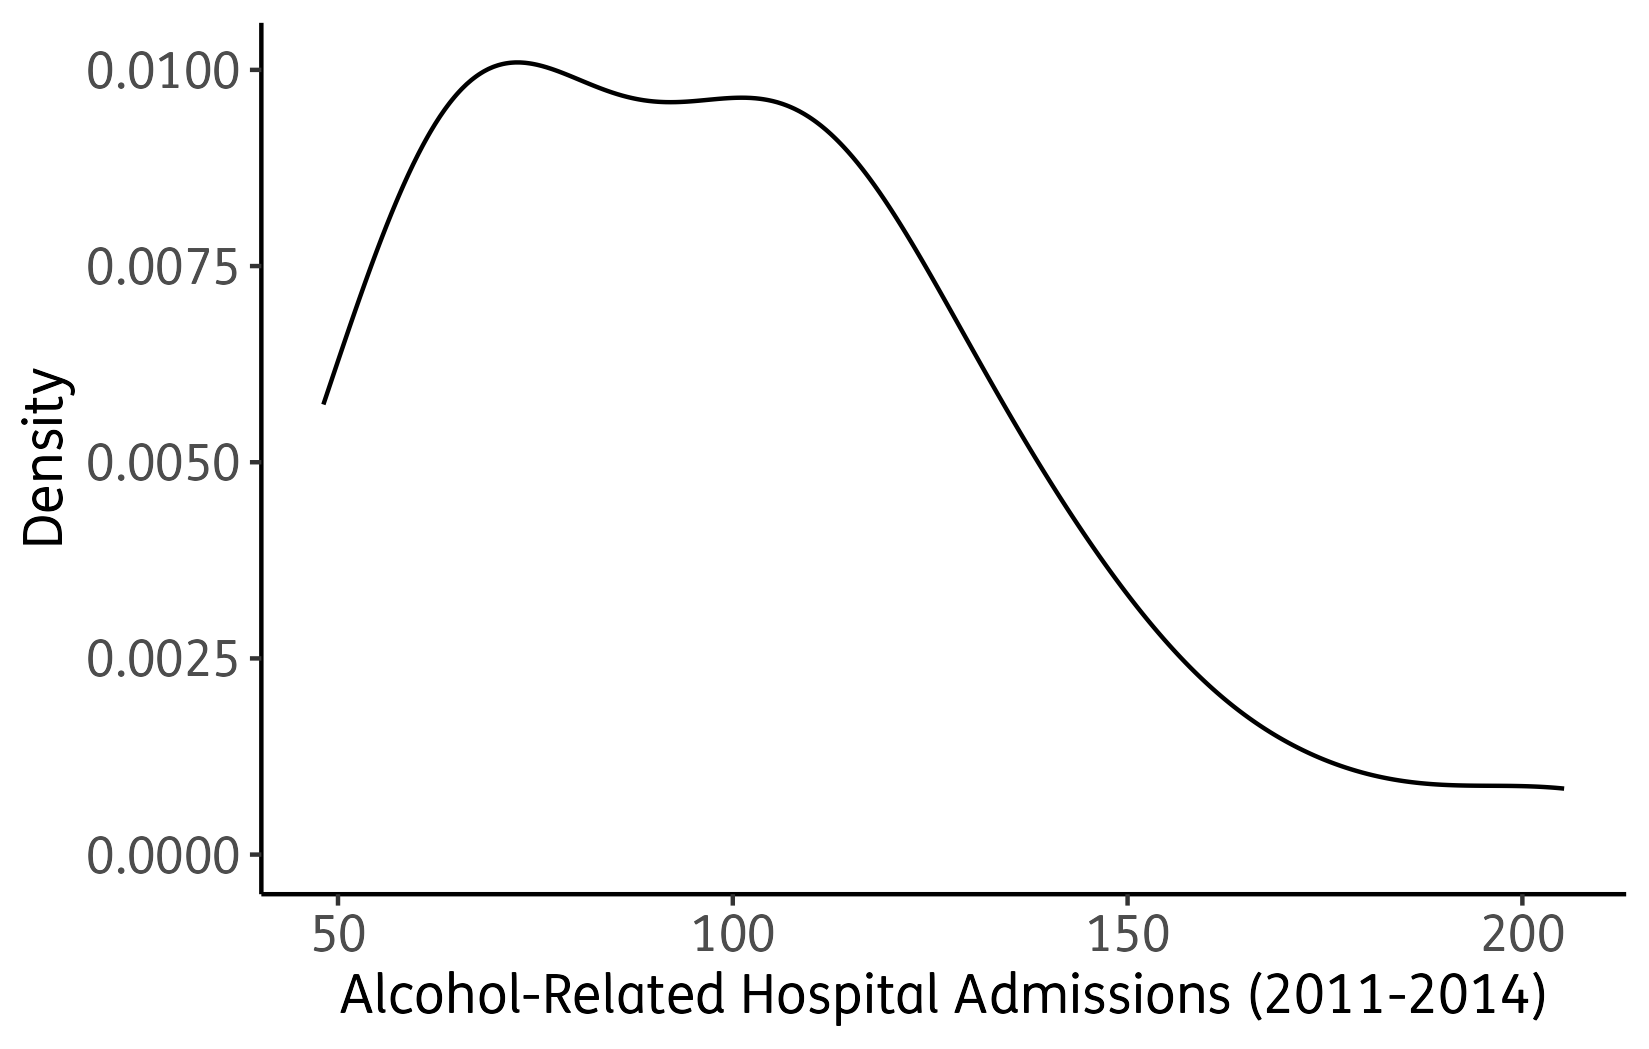
\includegraphics[width=0.5\linewidth,height=\textheight,keepaspectratio]{density.png}

}

\caption{\label{fig:dis_alc}Distribution of Alcohol-Related Hospital
Admissions (2011-2014)}

\end{figure}%

\normalsize

\begin{enumerate}
\def\labelenumi{\arabic{enumi}.}
\tightlist
\item
  Reproduce Figure \ref{fig:dis_alc}.
\item
  What does the distribution tell us about alcohol-related admissions to
  hospital?

  \begin{itemize}
   \item[]\begin{itemize}
       \item \textcolor{waraubergine}{Not perfectly normally distributed, with a positive skew.}
   \end{itemize}
  \end{itemize}
\item
  How does the shape of the distribution in Figure \ref{fig:dis_alc}
  relate to the descriptive statistics calculated in Section
  \ref{sec:descr}?

  \begin{itemize}
   \item[]\begin{itemize}
       \item \textcolor{waraubergine}{In a positvely skewed distribution the median is larger than the mean which is the case here. The maximum is also well above the third quartile.}
   \end{itemize}
  \end{itemize}
\item
  What would happen to the shape of the distribution if the median was
  smaller than the mean?

  \begin{itemize}
   \item[]\begin{itemize}
       \item \textcolor{waraubergine}{If they were identical, then this would be a normal distribution. If the median was smaller than the mean then we would be dealing with a negatively skewed distribution.}
   \end{itemize}
  \end{itemize}
\end{enumerate}

\subsection{Hypothesis}\label{hypothesis}

We are interested in how alcohol-related admissions to hospital have
affected mortality rates in Scotland. The following scatter plot uses
the variables \texttt{alc16} and \texttt{mortality20}.

\fontsize{7}{7}\selectfont

\begin{lstlisting}[language=R]
ggplot(simd, aes(alc16, mortality20)) +
  geom_point() +
  xlab('Alcohol-Related Hospital Admissions (2011-2014)') +
  ylab('Standardised Mortality Ratio (2014-2018)') +
  theme_classic() +
  theme(axis.text=element_text(size=12),
        axis.title=element_text(size=13)) 
\end{lstlisting}

\normalsize

\fontsize{7}{7}\selectfont
\normalsize

\fontsize{7}{7}\selectfont

\begin{figure}[H]

{\centering 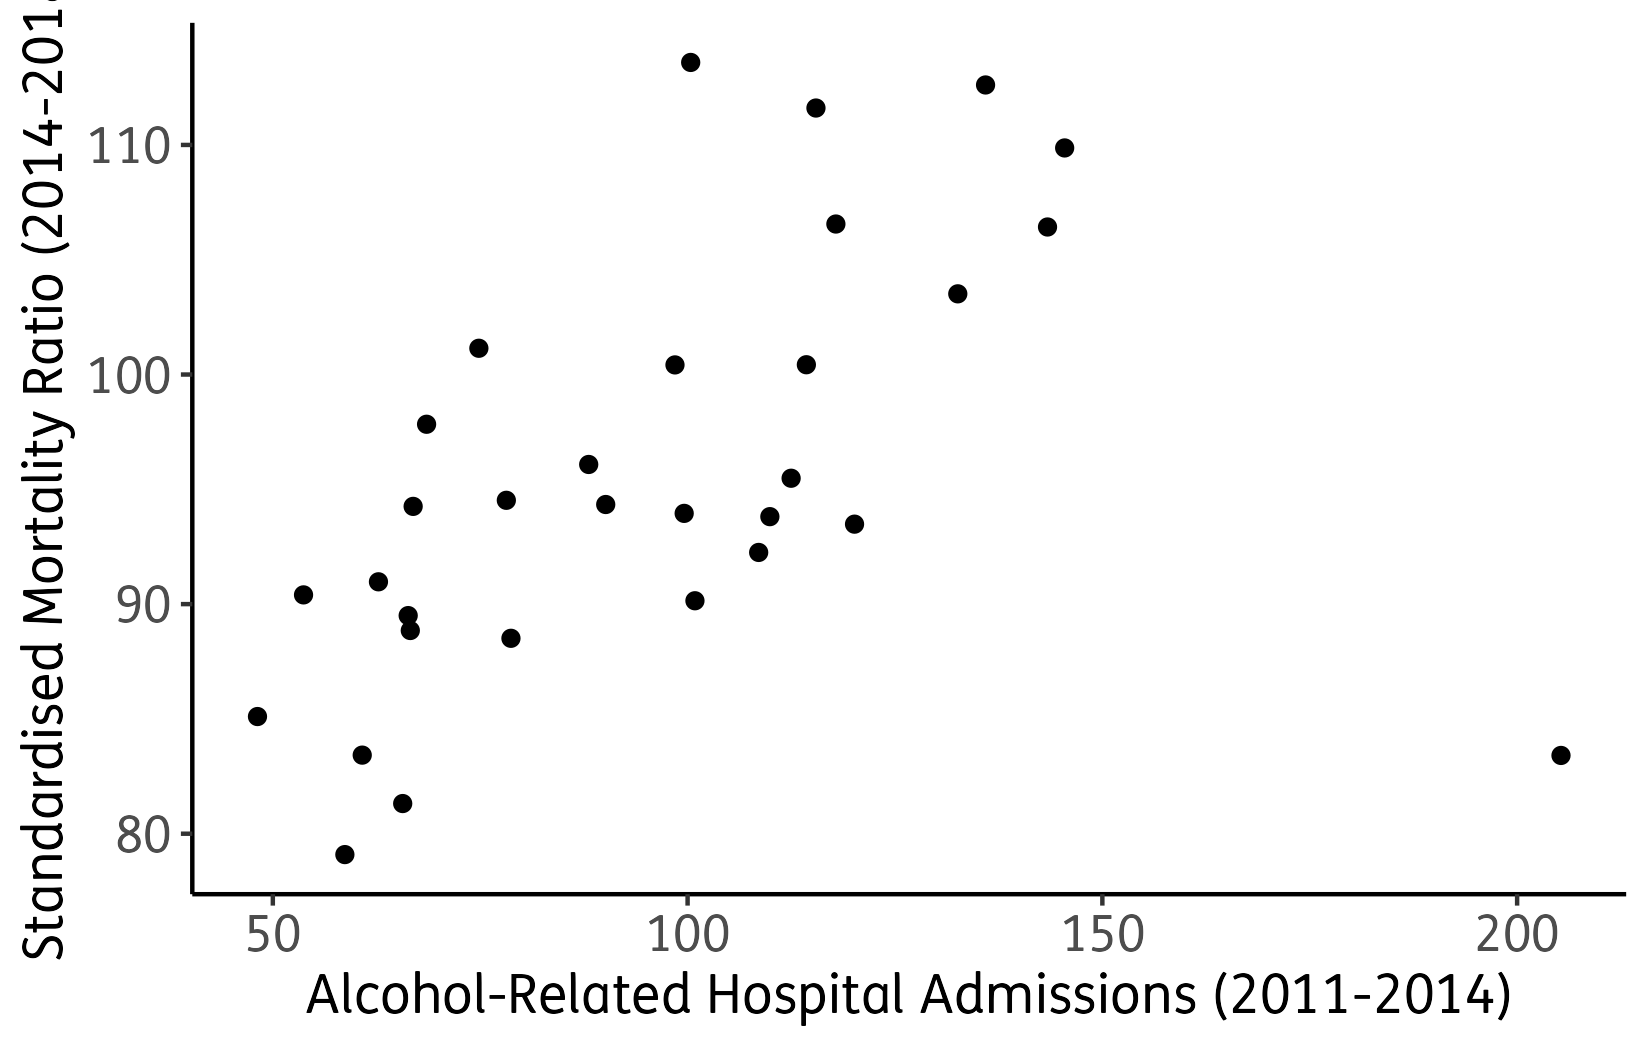
\includegraphics[width=0.5\linewidth,height=\textheight,keepaspectratio]{point.png}

}

\caption{\label{fig:causality}Alcohol-Related Hospital Admissions and
Mortality}

\end{figure}%

\normalsize

\begin{enumerate}
\def\labelenumi{\arabic{enumi}.}
\tightlist
\item
  Reproduce Figure \ref{fig:causality}.
\item
  Based on this scatter plot, formulate the alternative and the null
  hypotheses:
\end{enumerate}

~~~\textbf{H\(\pmb{_\text{A}}\):}
\textcolor{waraubergine}{The higher the rate of alcohol-related admissions to hospital between 2011 and 2014, the higher the standardised mortality ratio in 2014-2018.}\\
\strut \\
\strut ~~\textbf{H\(\pmb{_0}\):}
\textcolor{waraubergine}{The rate of alcohol-related admissions to hospital between 2011 and 2014 and the standardised mortality ratio in 2014-2018 are unrelated.}

\newpage

\subsection{Sampling}\label{sampling}

The data frame \texttt{simd} which we have been using so far represents
the population. Let us now draw a random sample of 15 councils as
follows:

\fontsize{7}{7}\selectfont

\begin{lstlisting}[language=R]
set.seed(6)
sample <- sample_n(simd, 15)
\end{lstlisting}

\normalsize

\begin{enumerate}
\def\labelenumi{\arabic{enumi}.}
\tightlist
\item
  Explain the purpose of the \texttt{set.seed} function.

  \begin{itemize}
   \item[]\begin{itemize}
       \item \textcolor{waraubergine}{It creates a pseudo-random number.}
   \end{itemize}
  \end{itemize}
\end{enumerate}

\subsection{Inferential Statistics}\label{inferential-statistics}

Let us now see if the mortality ratio has changed between the two waves
of 2016 and 2020. This is the worked example from the lecture, but I am
repeating it here deliberately, so that you can carry out the example
yourself.

\begin{enumerate}
\def\labelenumi{\arabic{enumi}.}
\tightlist
\item
  As a first step, create a new variable measuring the difference
  between \texttt{mortality20} and \texttt{mortality16}. Make sure that
  increases are positive and decreases negative.
\end{enumerate}

\fontsize{7}{7}\selectfont

\begin{lstlisting}[language=R]
sample$diff <- with(sample, mortality20-mortality16)
\end{lstlisting}

\normalsize

\begin{enumerate}
\def\labelenumi{\arabic{enumi}.}
\setcounter{enumi}{1}
\tightlist
\item
  What is the sample mean of the differences in mortality rates,
  variable \texttt{diff}?
\end{enumerate}

\fontsize{7}{7}\selectfont

\begin{lstlisting}[language=R]
summary(sample$diff)
##    Min. 1st Qu.  Median    Mean 3rd Qu.    Max. 
## -2.9276 -0.1155  1.5762  0.9063  2.2114  2.8747
\end{lstlisting}

\normalsize

\begin{enumerate}
\def\labelenumi{\arabic{enumi}.}
\setcounter{enumi}{2}
\tightlist
\item
  The sample size of 15 is small. Will it be appropriate to conduct a
  t-test? Why? Why not?

  \begin{itemize}
   \item[]\begin{itemize}
       \item \textcolor{waraubergine}{Yes, as the population distribution is likely to be normal.}
   \end{itemize}
  \end{itemize}
\item
  Find out whether the difference in mortality rates is significantly
  different from zero.
\end{enumerate}

\fontsize{7}{7}\selectfont

\begin{lstlisting}[language=R]
t.test(sample$diff, mu=0,  
       data=sample)
## 
##  One Sample t-test
## 
## data:  sample$diff
## t = 1.9689, df = 14, p-value = 0.06909
## alternative hypothesis: true mean is not equal to 0
## 95 percent confidence interval:
##  -0.08096415  1.89353389
## sample estimates:
## mean of x 
## 0.9062849
\end{lstlisting}

\normalsize

\begin{itemize}
    \item[]\begin{itemize}
        \item \textcolor{waraubergine}{There is no statistically significant difference in mortality ratios between the two waves.}
    \end{itemize}
\end{itemize}

\newpage

\begin{enumerate}
\def\labelenumi{\arabic{enumi}.}
\setcounter{enumi}{4}
\tightlist
\item
  Draw a graph which depicts the direction of the alternative hypothesis
  and the p-value. Try not to look at the lecture
  slides.\label{ex:testdiff}
\end{enumerate}

\fontsize{7}{7}\selectfont
\normalsize

\fontsize{7}{7}\selectfont

\begin{figure}[H]

{\centering 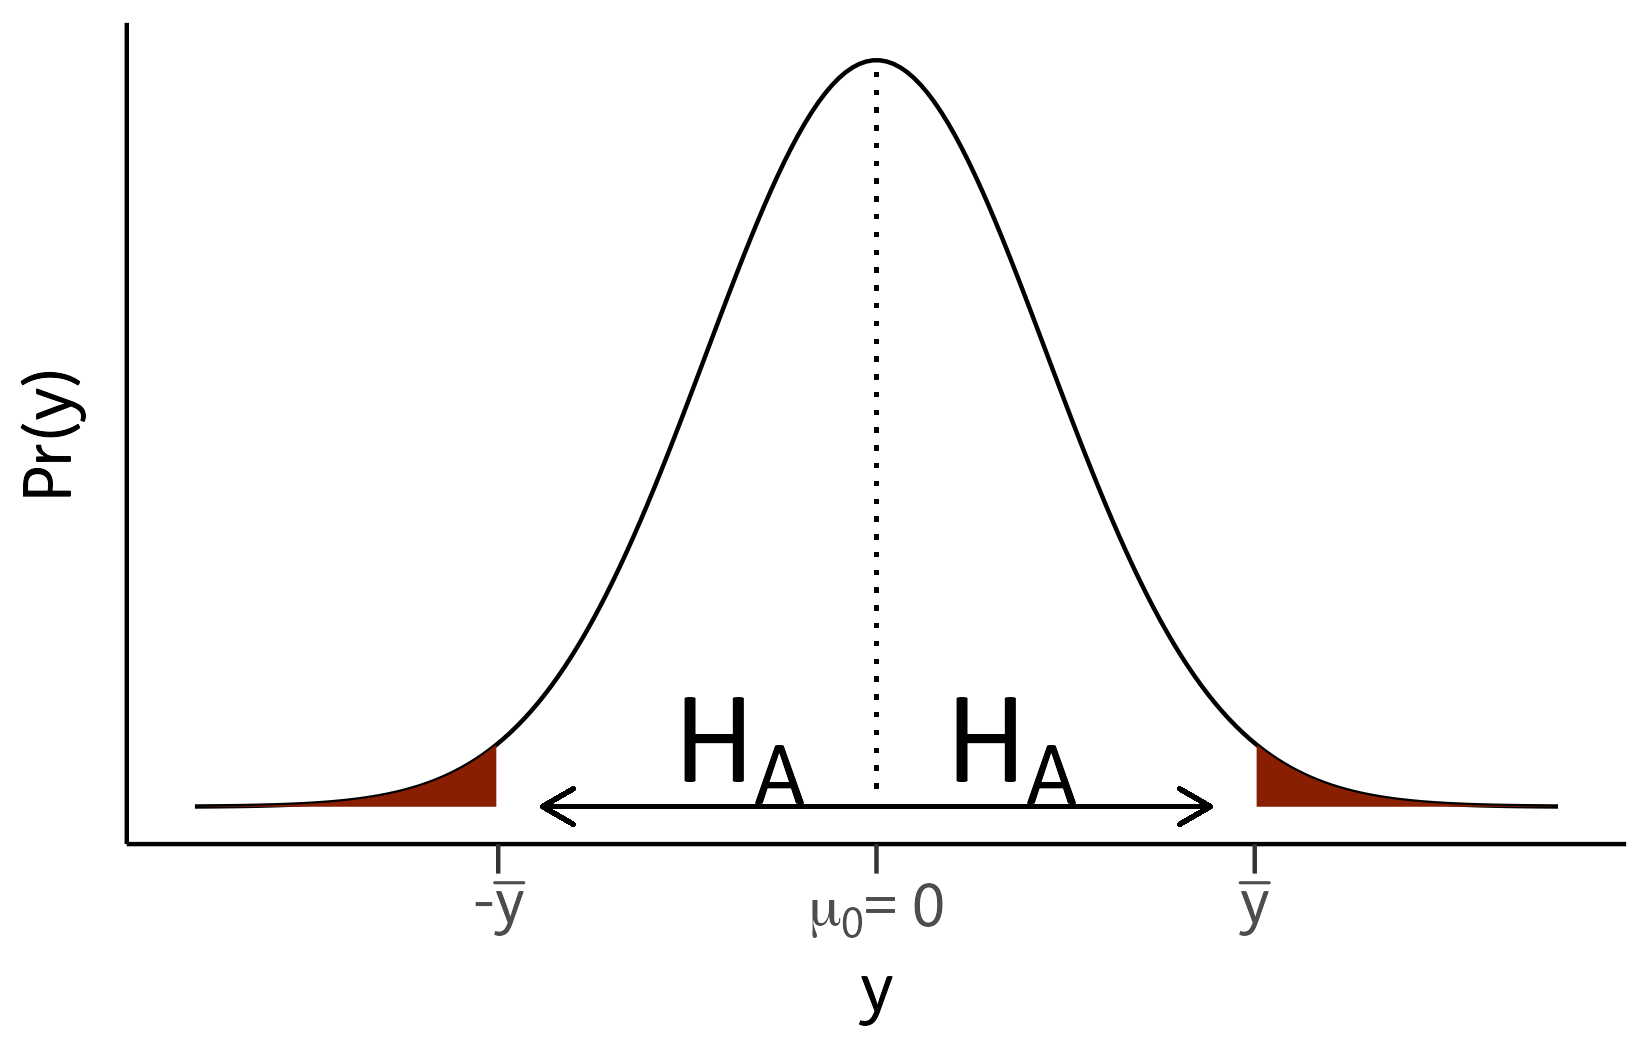
\includegraphics[width=0.5\linewidth,height=\textheight,keepaspectratio]{ha.png}

}

\caption{\label{fig:twosided}Two-Sided Significance Test}

\end{figure}%

\normalsize

\begin{enumerate}
\def\labelenumi{\arabic{enumi}.}
\setcounter{enumi}{5}
\tightlist
\item
  Suppose the Scottish Government claims that mortality rates have
  decreased. Test this claim.
\end{enumerate}

\fontsize{7}{7}\selectfont

\begin{lstlisting}[language=R]
t.test(sample$diff, mu=0,  
       data=sample,
       alternative = "less")
## 
##  One Sample t-test
## 
## data:  sample$diff
## t = 1.9689, df = 14, p-value = 0.9655
## alternative hypothesis: true mean is less than 0
## 95 percent confidence interval:
##      -Inf 1.717019
## sample estimates:
## mean of x 
## 0.9062849
\end{lstlisting}

\normalsize

\begin{itemize}
    \item[]\begin{itemize}
        \item \textcolor{waraubergine}{Absolutely not!}
    \end{itemize}
\end{itemize}

\begin{enumerate}
\def\labelenumi{\arabic{enumi}.}
\setcounter{enumi}{6}
\tightlist
\item
  Again, draw a graph which depicts the direction of the alternative
  hypothesis and the p-value. Try not to look at the lecture
  slides.\label{ex:testless}
\end{enumerate}

\fontsize{7}{7}\selectfont
\normalsize

\fontsize{7}{7}\selectfont

\begin{figure}[H]

{\centering 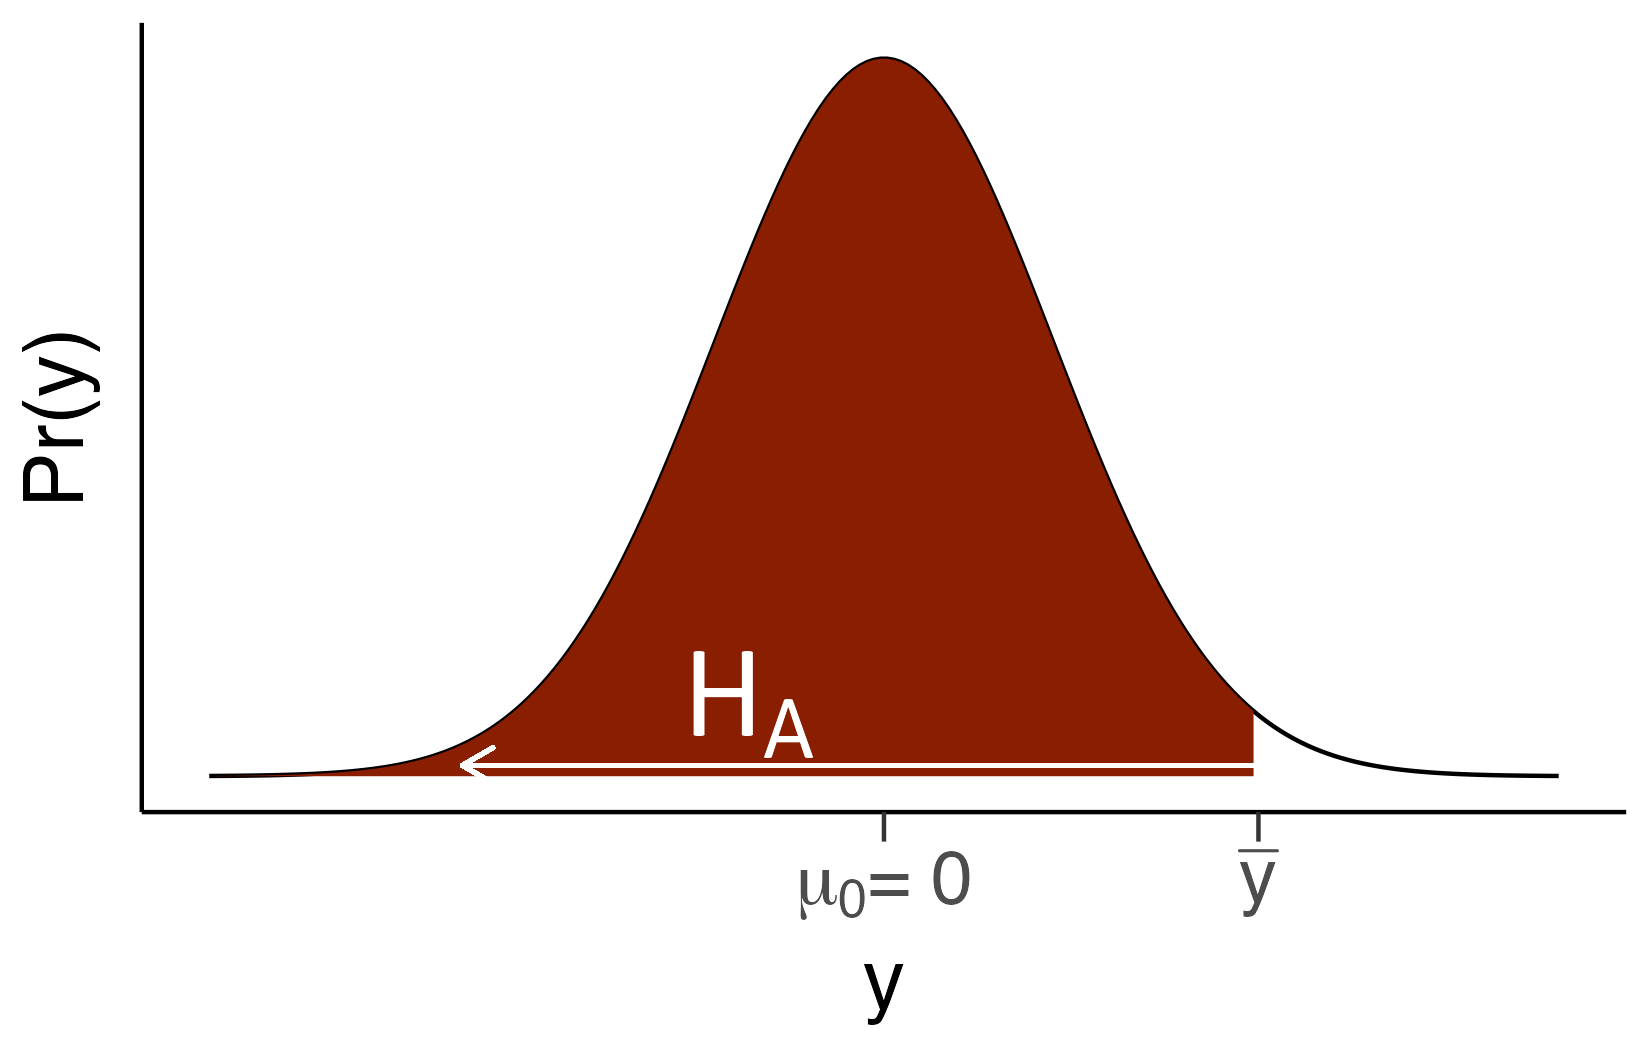
\includegraphics[width=0.5\linewidth,height=\textheight,keepaspectratio]{left.png}

}

\caption{\label{fig:leftsided}Left-Sided Significance Test}

\end{figure}%

\normalsize

\newpage

\begin{enumerate}
\def\labelenumi{\arabic{enumi}.}
\setcounter{enumi}{7}
\tightlist
\item
  Drawing on the results from Exercises \ref{ex:testdiff} and
  \ref{ex:testless}, reason about the p-value you would obtain if you
  tested the hypothesis that mortality rates have increased between the
  waves of 2016 and 2020.

  \begin{itemize}
   \item[]\begin{itemize}
       \item \textcolor{waraubergine}{Using Figure \ref{fig:leftsided}, the p-value for a right-sided test is indicated by the remaining white area. This area must be half of the blue area in Figure \ref{fig:twosided}. $\frac{0.06909}{2}=0.03454$. You can confirm this with:}
   \end{itemize}
  \end{itemize}
\end{enumerate}

\fontsize{7}{7}\selectfont

\begin{lstlisting}[language=R]
t.test(sample$diff, mu=0,  
       data=sample,
       alternative = "greater")
## 
##  One Sample t-test
## 
## data:  sample$diff
## t = 1.9689, df = 14, p-value = 0.03454
## alternative hypothesis: true mean is greater than 0
## 95 percent confidence interval:
##  0.09555077        Inf
## sample estimates:
## mean of x 
## 0.9062849
\end{lstlisting}

\normalsize

\begin{itemize}
    \item[]\begin{itemize}
        \item \textcolor{waraubergine}{This is significant. Mortality rates have indeed increased.}
    \end{itemize}
\end{itemize}

\subsection{Causality}\label{causality}

\begin{enumerate}
\def\labelenumi{\arabic{enumi}.}
\tightlist
\item
  Identify the elements of symmetry and asymmetry in the setup of this
  case study.
\end{enumerate}

\begin{itemize}
\item[]\begin{itemize}
  \item \textcolor{waraubergine}{Symmetry: Alcohol abuse leads to health issues and possibly death. It's not really a theory, but medical reasoning.}
  \item \textcolor{waraubergine}{Asymmetry: I have taken the mortality from a later wave than the alcohol-related admissions to hospital. So, rverse causality is not possible, but bear in mind that a time-lag might be insufficient to justify asymmetry.}
\end{itemize}  \end{itemize}

\begin{enumerate}
\def\labelenumi{\arabic{enumi}.}
\setcounter{enumi}{1}
\tightlist
\item
  Consider again Figure \ref{fig:cause} from the lecture. Which aspects
  of establishing causality has the case study addressed? What is
  missing?
\end{enumerate}

\begin{itemize}
\item[]\begin{itemize}
  \item \textcolor{waraubergine}{Practically everything is still missing, bar the theory and historical context, and perhaps asymmetry. We have not touched anything else in this graph, yet.}
\end{itemize} \end{itemize}

\fontsize{7}{7}\selectfont

\begin{figure}[H]

{\centering 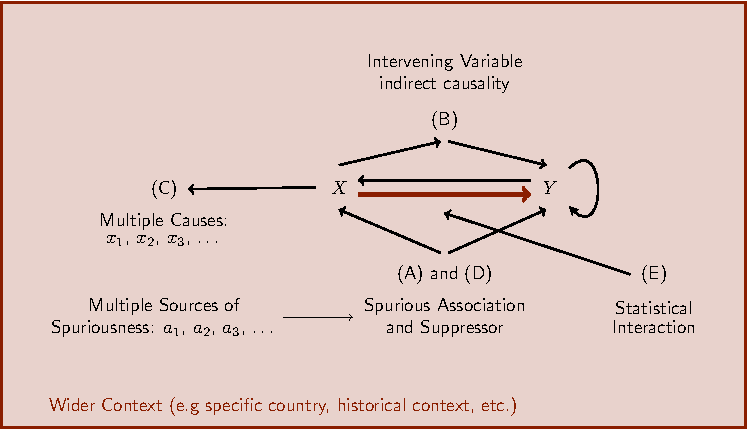
\includegraphics[width=0.75\linewidth,height=\textheight,keepaspectratio]{PO91Q_Seminar_Week-5_Solutions_files/figure-pdf/unnamed-chunk-21-1.pdf}

}

\caption{\label{fig:cause}Causality Framework}

\end{figure}%

\normalsize


\printbibliography[title=List of References]


\end{document}
